\chapter{Plots of the results}
\label{app:Results}
\section{Capacitors at D=0.6}
\begin{figure}[H]
	\centering
	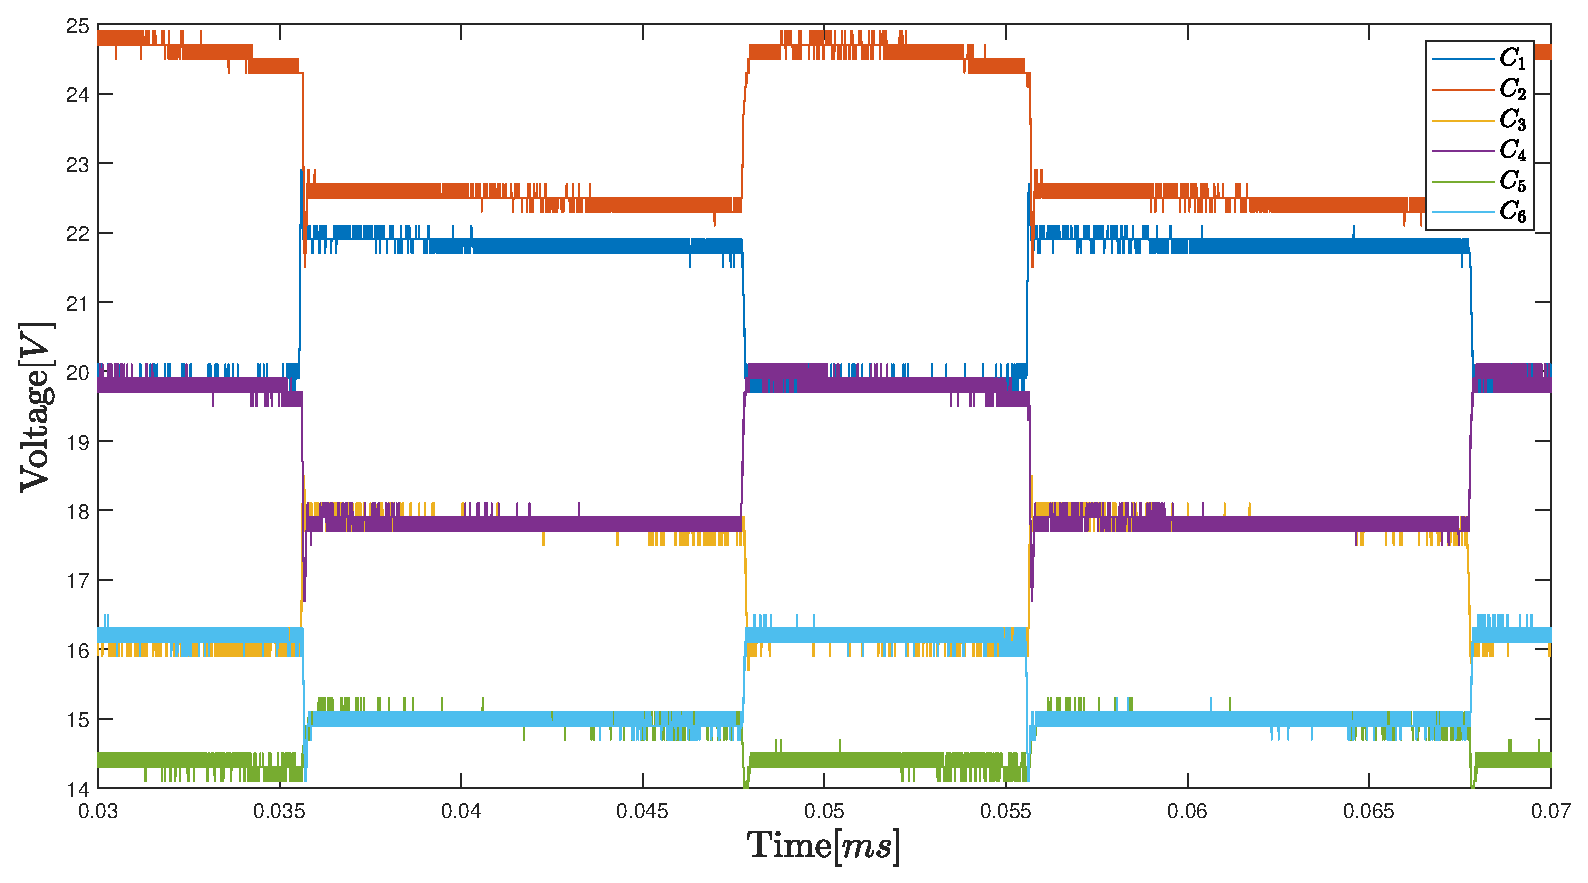
\includegraphics[width=\textwidth]{figures/06Testing/botcap60per.eps}
	\caption{Bottom capacitors}
\end{figure}
\vspace{10mm}
\begin{figure}[H]
	\centering
	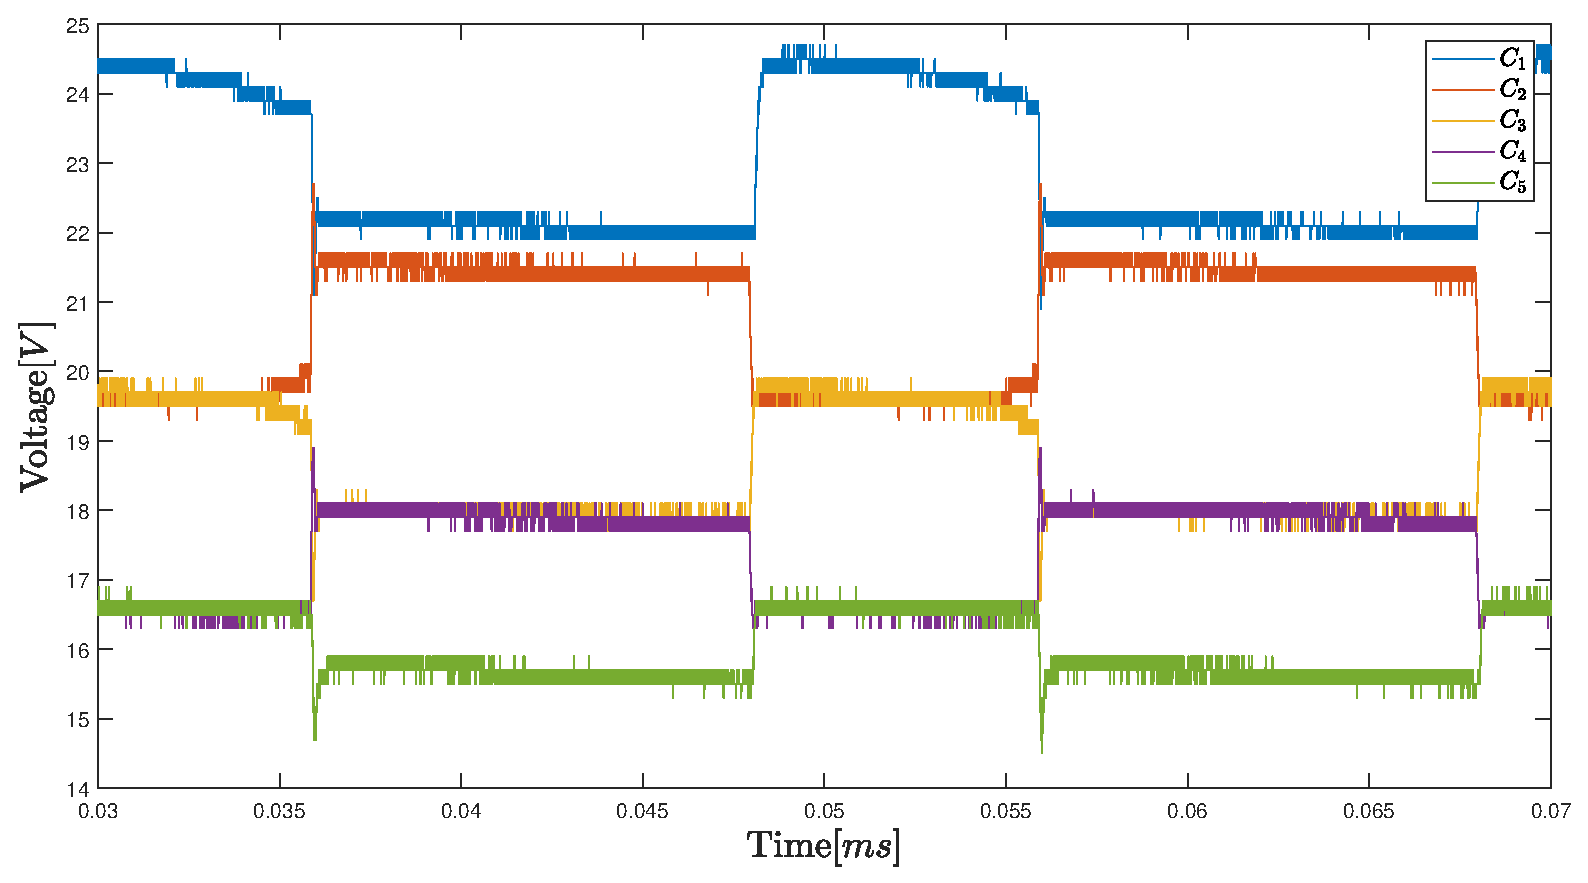
\includegraphics[width=\textwidth]{figures/06Testing/topcap60per.eps}
	\caption{Top capacitors}
\end{figure}
\section{Inductors at D=0.6}
\begin{figure}[H]
	\centering
	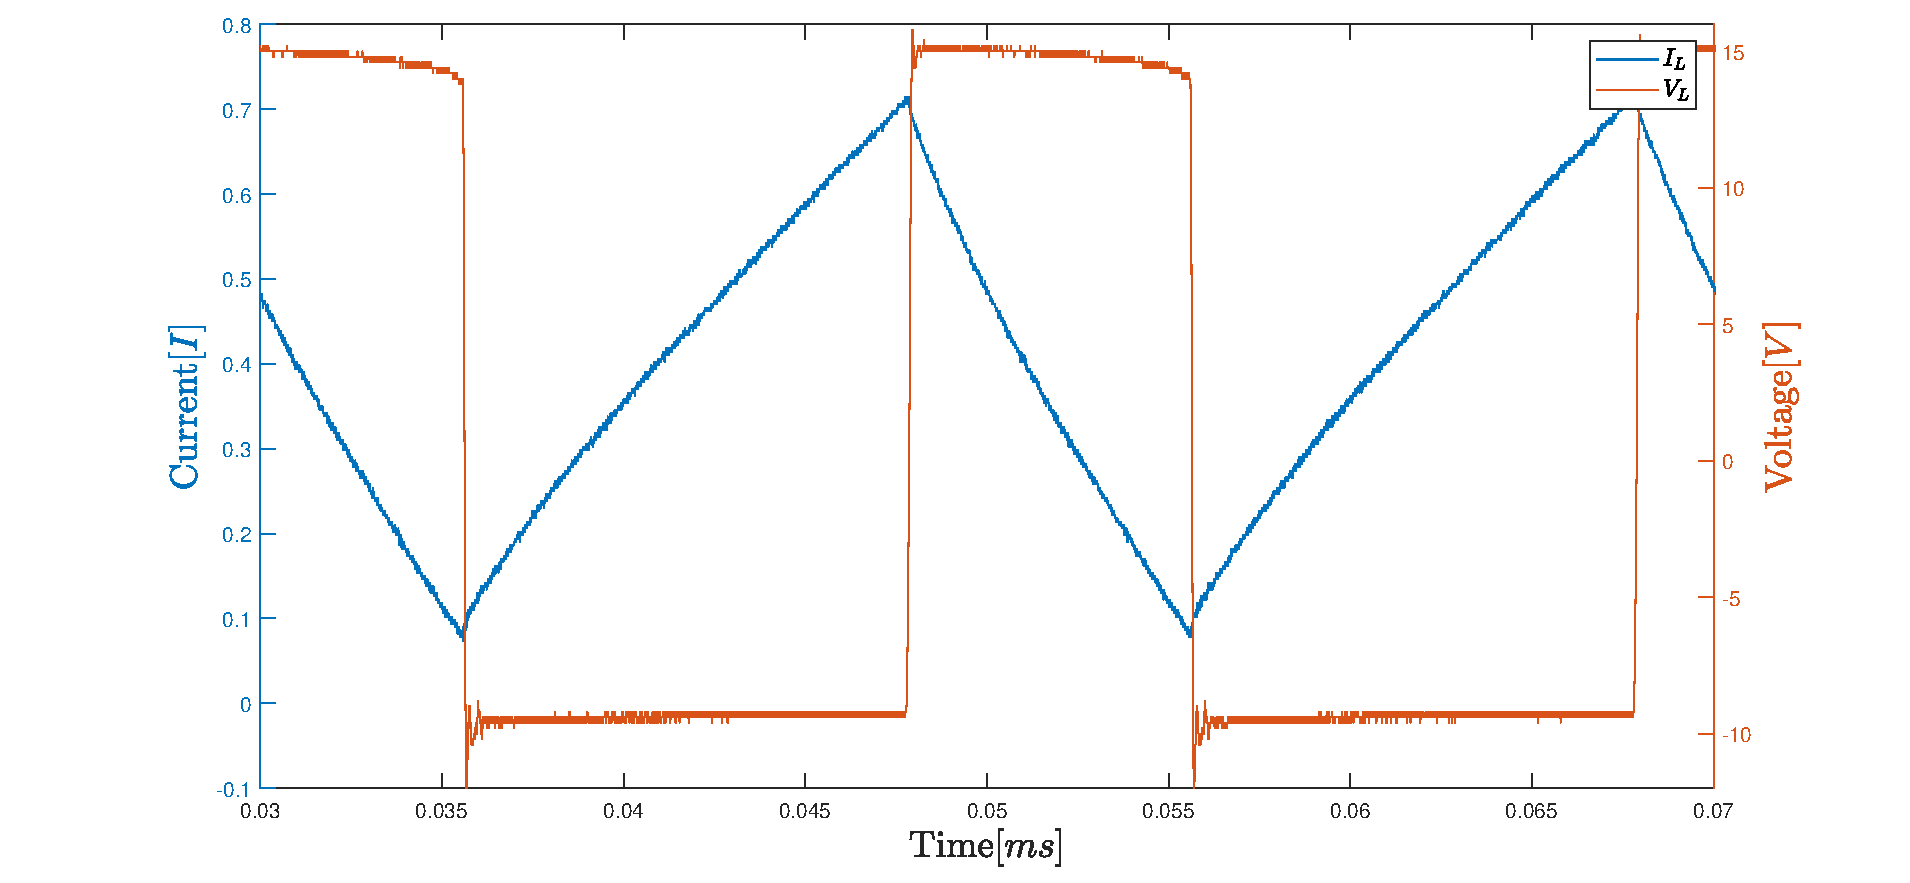
\includegraphics[width=\textwidth]{figures/06Testing/botind60per.eps}
	\caption{Bottom inductor}
\end{figure}
\begin{figure}[H]
	\centering
	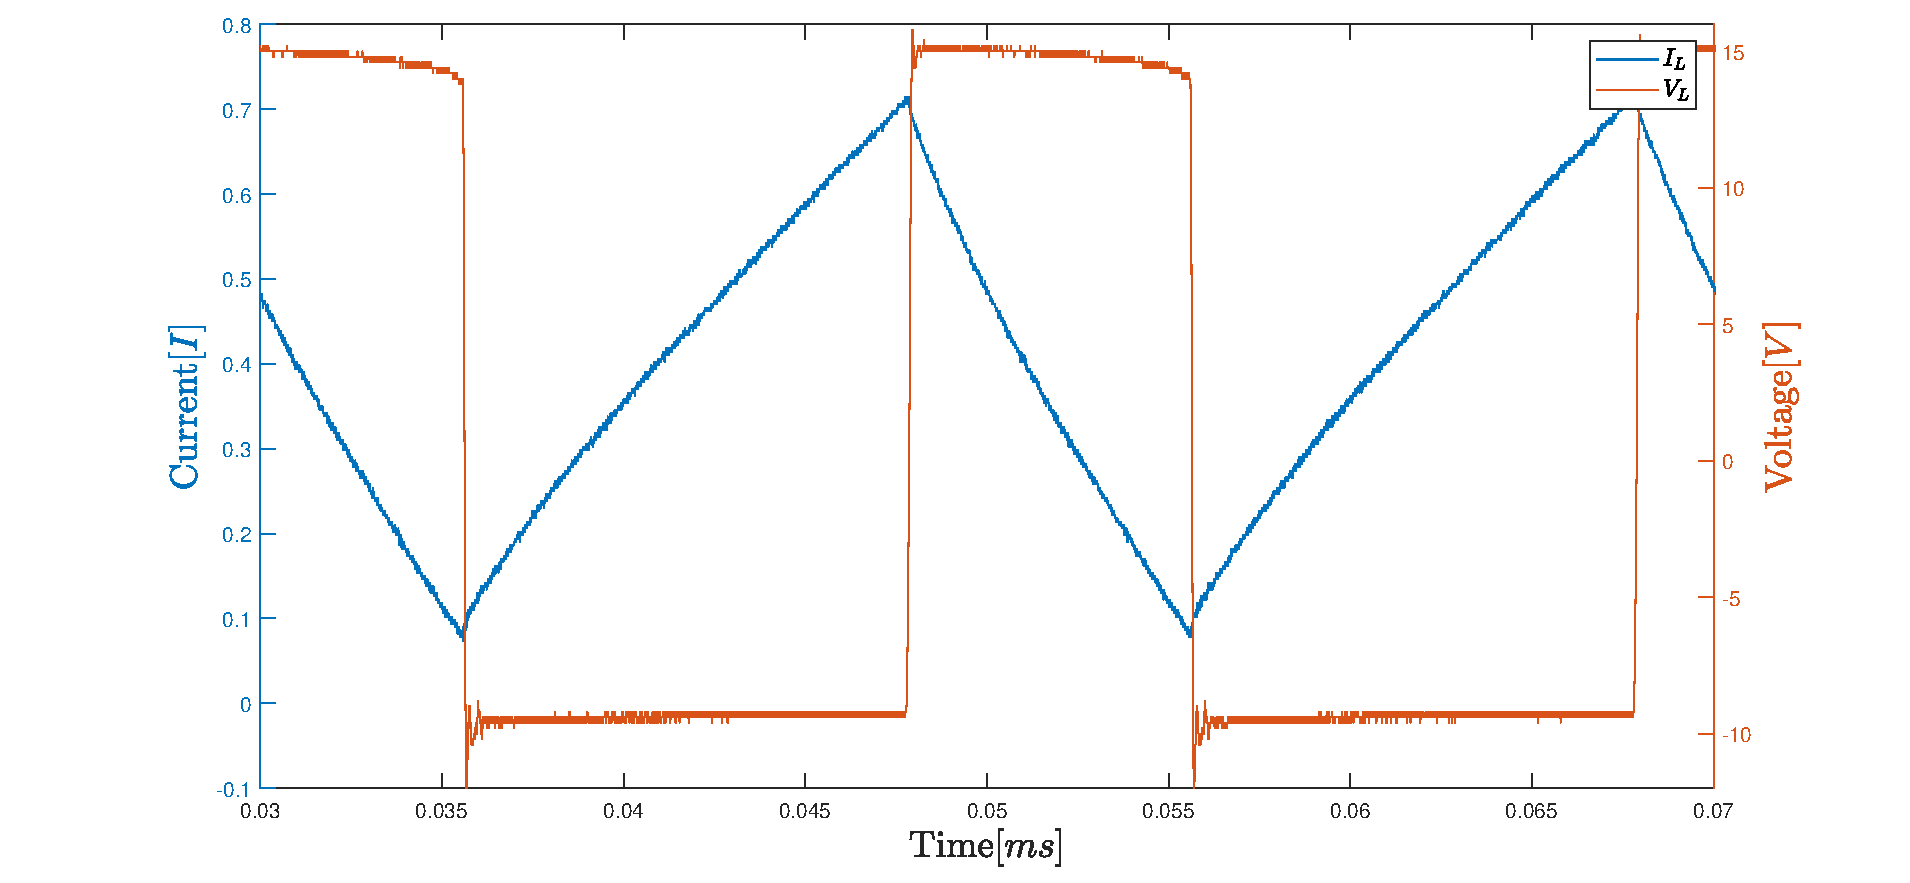
\includegraphics[width=\textwidth]{figures/06Testing/botind60per.eps}
	\caption{Top inductor}
\end{figure}
\section{Diodes at D=0.6}
\begin{figure}[H]
	\centering
	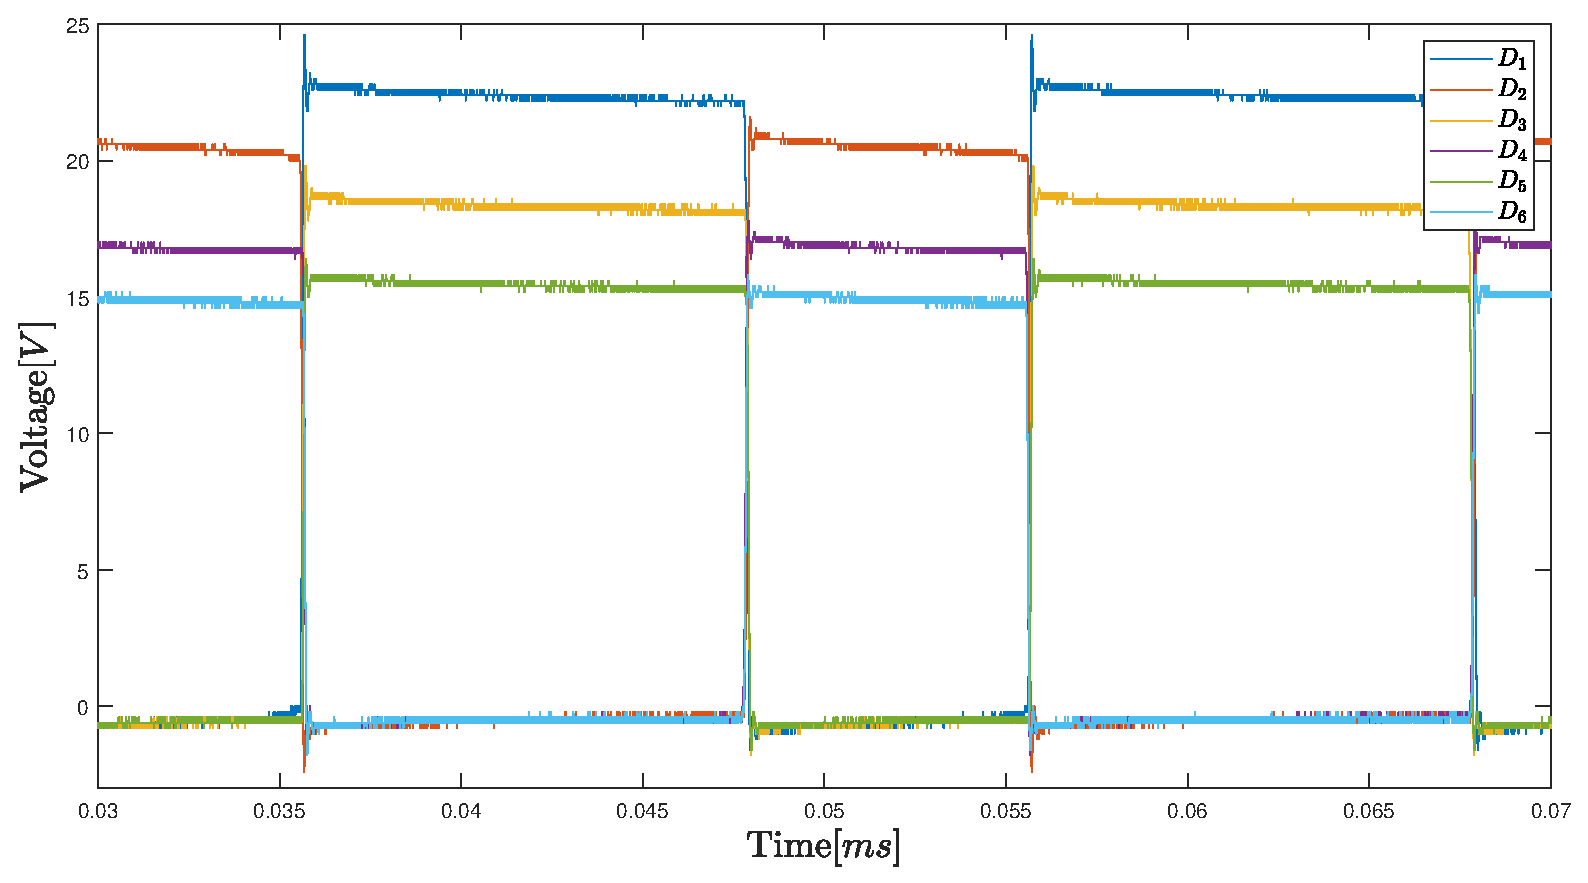
\includegraphics[width=\textwidth]{figures/06Testing/botdio60per.eps}
	\caption{Bottom diodes}
\end{figure}
\begin{figure}[H]
	\centering
	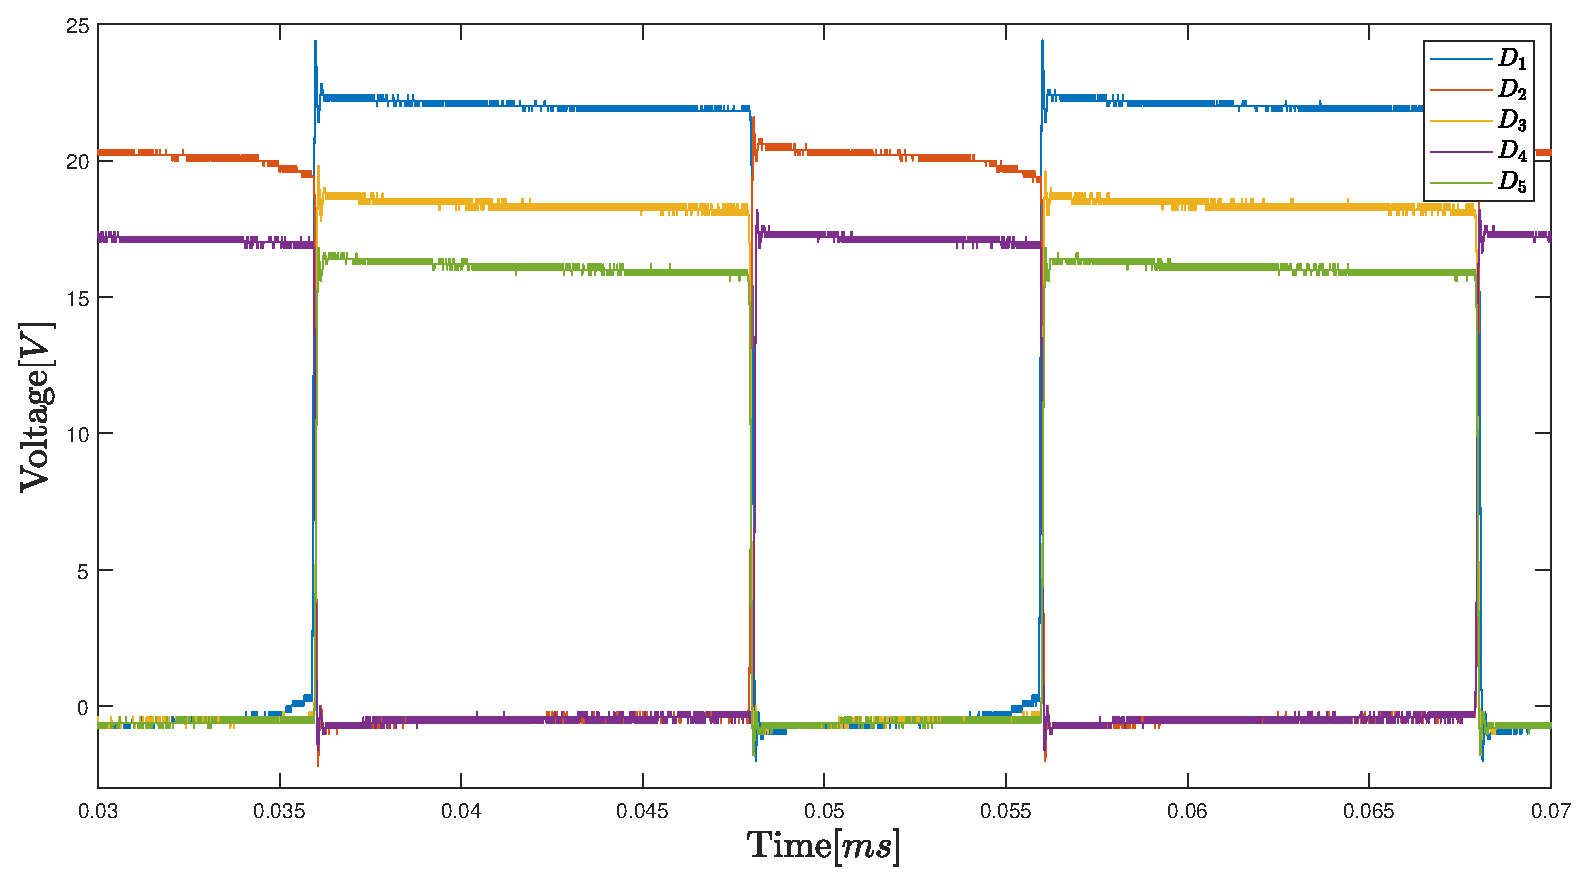
\includegraphics[width=\textwidth]{figures/06Testing/topdio60per.eps}
	\caption{Top diodes}
\end{figure}

\section{MOSTEFs at D=0.6}
\begin{figure}[H]
	\centering
	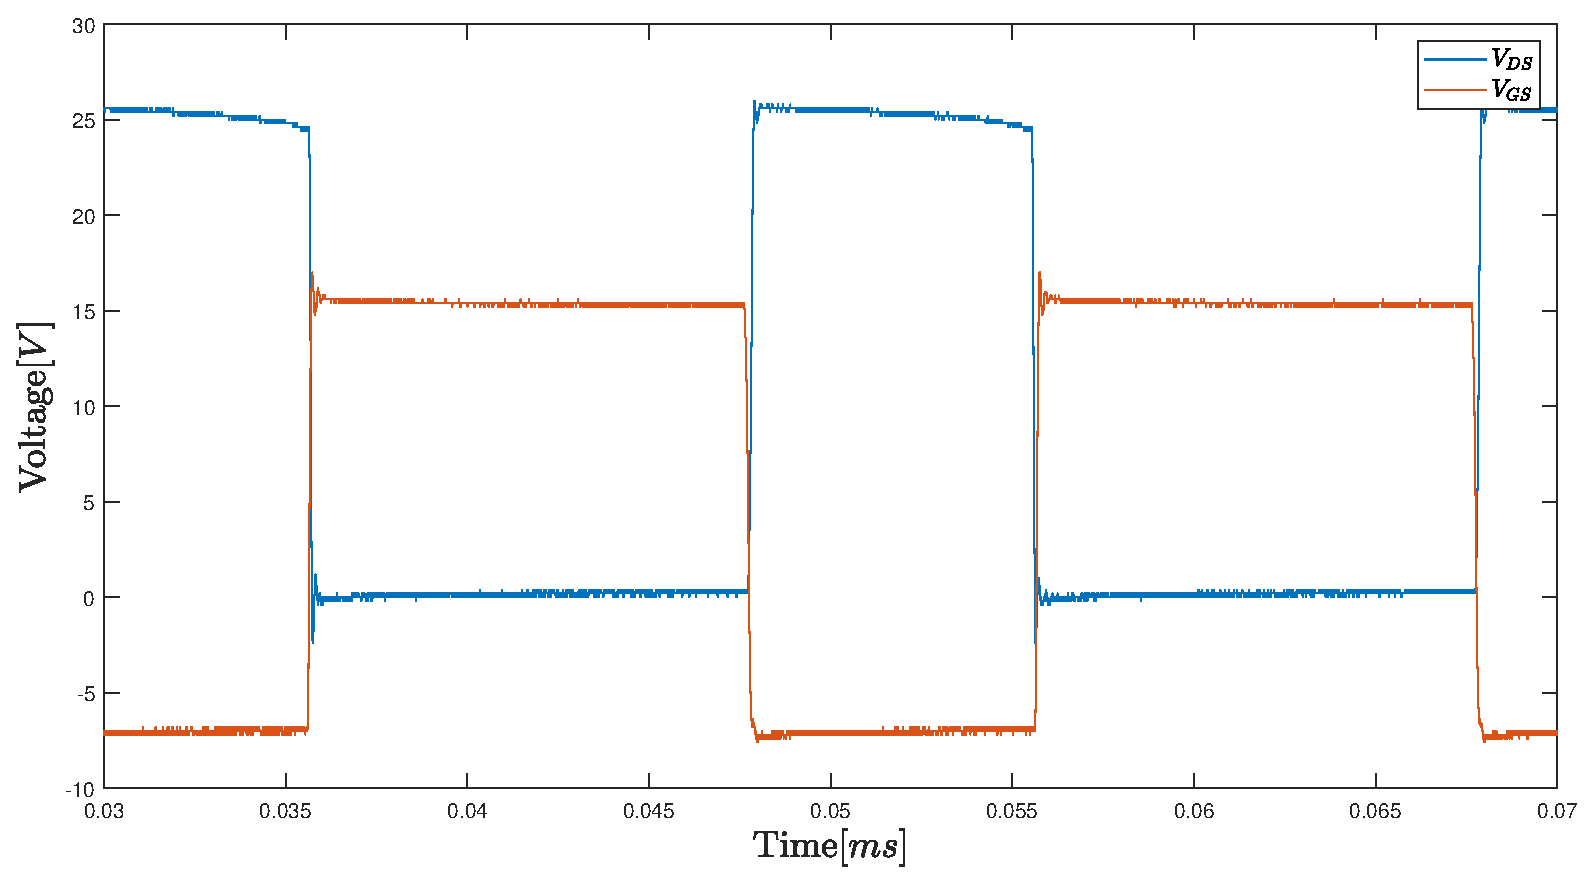
\includegraphics[width=\textwidth]{figures/06Testing/botswi60per.eps}
	\caption{Bottom MOSFET}
\end{figure}

\begin{figure}[H]
	\centering
	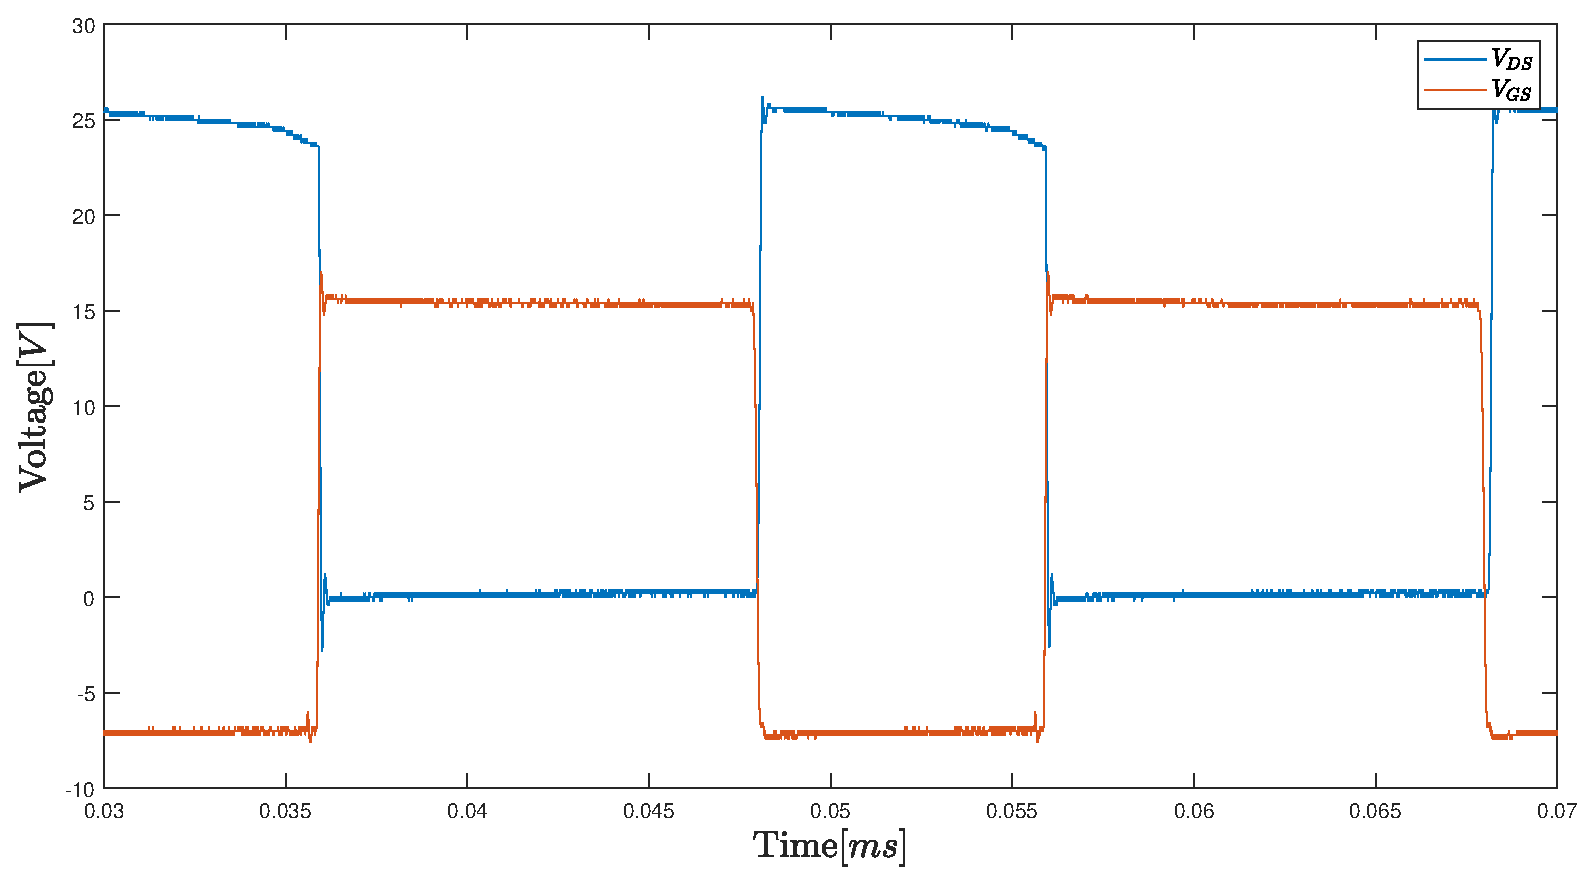
\includegraphics[width=\textwidth]{figures/06Testing/topswi60per.eps}
	\caption{Top MOSFET}
\end{figure}